\documentclass{article}

\usepackage[utf8]{inputenc}
\usepackage[T1]{fontenc}
\usepackage[frenchb]{babel}
\usepackage{tikz}
\usepackage{amsmath}
\usetikzlibrary{chains,positioning,matrix,arrows,decorations,calc}




\setlength{\parindent}{0pt}
\setlength{\parskip}{2ex}

\newcounter{exocount}
\setcounter{exocount}{0}

\newcounter{enoncecount}
\setcounter{enoncecount}{0}
\newenvironment{enonce}
{% This is the begin code
\stepcounter{enoncecount}
\bf\small \arabic{enoncecount}.
\begin{bf}
}
{% This is the end code
\end{bf}
}


\newcounter{sousenoncecount}
\setcounter{sousenoncecount}{0}
\newenvironment{sousenonce}
{% This is the begin code
\stepcounter{sousenoncecount}
\bf\small (\alph{sousenoncecount})
\begin{bf}
}
{% This is the end code
\end{bf}
}



\begin{document}
\title{Rapport de projet : FMIN105 -- Cours algorithmique/complexité/calculabilité}
\author{Bertrand BRUN \\ Yohann \\ John CHARRON \\ Georges DUPERON}
\date
\maketitle

\tableofcontents
\newpage

\section{Descriptif des tâches}
Vos résultats seront présentés en procédant à la rédaction d'un mémoire dont la qualité influencera la note finale. Ce manuscrit sera rendu le jour de la soutenance. La soutenance consiste à présenter résultats pratiques (choix du langage, choix des structures de données, résultats obtenus, tests sur un grand jeu de données, analyse de ceux-ci ...) Vous aurez 15 minutes au maximum, questions comprises. Vous avez la possibilité d'utiliser des transparents.


\section{Partie théorique}
\subsection{Partie algorithmique}

\subsubsection*{Exercice \stepcounter{exocount}\bf\small \arabic{exocount} -- Modélisation et résolution d'un problème d'ordonnancement par un problème de flot maximum : ordonnancement avec coûté dépendants des dates de début}
\addcontentsline{toc}{section}{Exercice \arabic{exocount} -- Modélisation et résolution d'un problème d'ordonnancement par un problème de flot maximum : ordonnancement avec coûté dépendants des dates de début}



\begin{figure}[h!]
  \centering
  \begin{tikzpicture}[node distance=3cm]
    \node (J1) {$J_{1}$};
    \node (J2) [above of=J1] {$J_{2}$};
    \node (J3) [right of=J1] {$J_{3}$};
    \draw[->] (J1) -- (J2);
    \draw[->] (J1) -- (J3);
    \draw[->] (J3) -- (J2);
  \end{tikzpicture}
  \caption{Graphe G}
  \label{fig:graphe-g}
\end{figure}

\begin{enonce}
Construire le graphe $G*$ pour $n = 3$, $T = 5$, $p_1 = 1$, $p_2 = 2$, $p_3 = 1$, 
$E = \{(1,2), (1,3), (3,2)\}$ et les coûts suivants :
\end{enonce}

\begin{figure}[h!]
  \centering
	\begin{tabular}{cccccc}
	\hline	
	$i,t$ & 0 & 1 & 2 & 3 & 4\\
	\hline
	1 & 0 & 2 & 5 & 0 & 1\\
	2 & 1 & 1 & 2 & 4 & -\\
	3 & 1 & 10 & 2 & 3 & 3\\
	\hline
\end{tabular}
\end{figure}

\begin{figure}[h!]
  \centering
  \colorlet{affectation}{green!50!black}
  \colorlet{auxiliaire}{black}
  \colorlet{précédence}{blue}
  \begin{tikzpicture}[
      affectation/.style = {
        draw=affectation,
        ->
      },
      auxiliaire/.style = {
        draw=auxiliaire,
        ->
      },
      précédence/.style = {
        draw=précédence,
        ->
      },
      capacité/.style = {
        fill=white,
        font=\footnotesize
      },
      capacité affectation/.style = {
        text=affectation,
        capacité
      },
      capacité auxiliaire/.style = {
        text=auxiliaire,
        capacité
      },
      capacité précédence/.style = {
        text=précédence,
        capacité
      }
    ]
    
    \matrix[matrix of math nodes, nodes in empty cells, row sep=1cm, column sep=1cm] (m) {
      & v_{1,0} & v_{1,1} & v_{1,2} & v_{1,3} & v_{1,4} & v_{1,5} & \\
      s & v_{3,0} & v_{3,1} & v_{3,2} & v_{3,3} & v_{3,4} & v_{3,5} & t \\
      & v_{2,0} & v_{2,1} & v_{2,2} & v_{2,3} & v_{2,4} & & \\
    };
    
    %% Penser a rajouter les J1, J2 et J3 a gauche du graphe.
    
  	\draw[affectation] (m-1-2)-- node[capacité affectation]{0} (m-1-3);
	\draw[affectation] (m-1-3)-- node[capacité affectation]{2} (m-1-4);
	\draw[affectation] (m-1-4)-- node[capacité affectation]{5} (m-1-5);
	\draw[affectation] (m-1-5)-- node[capacité affectation]{0} (m-1-6);
	\draw[affectation] (m-1-6)-- node[capacité affectation]{1} (m-1-7);

	\draw[affectation] (m-2-2)-- node[capacité affectation]{1} (m-2-3);
	\draw[affectation] (m-2-3)-- node[capacité affectation]{10} (m-2-4);
	\draw[affectation] (m-2-4)-- node[capacité affectation]{2} (m-2-5);
	\draw[affectation] (m-2-5)-- node[capacité affectation]{3} (m-2-6);
	\draw[affectation] (m-2-6)-- node[capacité affectation]{3} (m-2-7);

	\draw[affectation] (m-3-2)-- node[capacité affectation]{1} (m-3-3);
	\draw[affectation] (m-3-3)-- node[capacité affectation]{1} (m-3-4);
	\draw[affectation] (m-3-4)-- node[capacité affectation]{2} (m-3-5);
	\draw[affectation] (m-3-5)-- node[capacité affectation]{4} (m-3-6);
	
  	\draw[auxiliaire] (m-2-1)-- node[capacité auxiliaire]{$\infty$} (m-1-2);
  	\draw[auxiliaire] (m-2-1)-- node[capacité auxiliaire]{$\infty$} (m-2-2);
  	\draw[auxiliaire] (m-2-1)-- node[capacité auxiliaire]{$\infty$} (m-3-2);
  	\draw[auxiliaire] (m-1-7)-- node[capacité auxiliaire]{$\infty$} (m-2-8);
  	\draw[auxiliaire] (m-2-7)-- node[capacité auxiliaire]{$\infty$} (m-2-8);
  	\draw[auxiliaire] (m-3-6)--(m-3-7.center)-- node[capacité auxiliaire]{$\infty$} (m-2-8);
	
	\draw[précédence] (m-1-2)-- node[capacité précédence]{$\infty$} (m-2-3);
	\draw[précédence] (m-1-3)-- node[capacité précédence]{$\infty$} (m-2-4);
	\draw[précédence] (m-1-4)-- node[capacité précédence]{$\infty$} (m-2-5);
	\draw[précédence] (m-1-5)-- node[capacité précédence]{$\infty$} (m-2-6);
	\draw[précédence] (m-1-6)-- node[capacité précédence]{$\infty$} (m-2-7);
    
	\draw[précédence] (m-2-2)-- node[capacité précédence]{$\infty$} (m-3-3);
	\draw[précédence] (m-2-3)-- node[capacité précédence]{$\infty$} (m-3-4);
	\draw[précédence] (m-2-4)-- node[capacité précédence]{$\infty$} (m-3-5);
	\draw[précédence] (m-2-5)-- node[capacité précédence]{$\infty$} (m-3-6);

	\draw[précédence] (m-1-2)-- node[capacité précédence,pos=0.3]{$\infty$} (m-3-3);
	\draw[précédence] (m-1-3)-- node[capacité précédence,pos=0.3]{$\infty$} (m-3-4);
	\draw[précédence] (m-1-4)-- node[capacité précédence,pos=0.3]{$\infty$} (m-3-5);
	\draw[précédence] (m-1-5)-- node[capacité précédence,pos=0.3]{$\infty$} (m-3-6);

  \end{tikzpicture}
  \caption{Graphe G*}
  \label{fig:graphe-g*}
\end{figure}



\begin{enonce}
Montrer qu'il existe une coupe dans G* de capacité minimale de laquelle sort un et un seul arc d'affectation par job.
\end{enonce}

Démonstration par construction~: 
On effectue un tri topologique sur le graphe des contraintes de précédence $G(\{J_1, \dots, J_n\}, E)$. Ce tri topologique nous donne un ensemble ordonné de n\oe uds $(J_{a1}, \dots, J_{an})$. On a donc~:
$$\forall J_{ai} \quad \not\exists \ j < i \quad | \quad \exists (J_{aj}, J_{ai}) \in E$$
On transforme ensuite $G$ en un graphe de flots à l'aide de l'algorithme fourni dans le sujet. 
Considérons les arcs entre les $v_{ai,t}$~: 
\begin{itemize}
	\item Arcs d'affectation~: ces arcs sont entre des sommets $v_{ai,t}$ et $v_{aj,t'}$ avec $ai = aj$
	\item Arcs de précédences~: ces arcs sont entre des sommets $v_{ai,t}$ et $v_{aj,t'}$ avec $ai < aj$, car grâce au tri topologique, il n'existe pas d'arcs entre des sommets $J_{ai}$ et $J_{aj}$ avec $aj < ai$, et de plus il n'y a pas de boucle (donc pas d'arc $(J_{ai},J_{ai})$ dans $G$, donc pas d'arc $(v_{ai,t}, v_{ai,t'})$ dans $G*$).
	\item Arcs auxiliaires~: ces arcs ne sont pas entre des sommets $v_{ai,t}$.
\end{itemize}
On va créer une $(s-t)-\mathrm{coupe}$ minimale. Etant donné que cette coupe est minimale, aucun arc de capacité infinie n'a son origine dans $S$ et son extremité dans $\overline{S}$.

TODO~: Montrons que s'il s'agit d'une coupe minimale, il ne sort qu'un et qu'un
seul arc d'affectation par job. Il faut aussi montrer qu'il (il = ?) existe.

\begin{enonce}
Montrer que l'on peut associer un ordonnancement réalisable (qui respectent toutes les contraintes à toute 
coupe de capacité finie minimale dans le graphe. Quel est le coût de cet ordonnancement ? 
\end{enonce}

TODO~: Attention à la phrase suivante, ce n'est pas tout à fait ce qu'on a montré dans l'exercice 2

Dans l'exercice précédent, on a montré que de toute coupe minimale sort un et un seul arc d'affectation par job.

On cherche à associer un ordonancement réalisable à toute coupe minimale.

On va construire cet ordonancement de la manière suivante~: à chaque
fois qu'un arc d'affectation $v_{i,t}, v_{i,t+1}$ traverse la coupe,
on exécute le job $i$ à l'instant $t$ dans l'ordonancement.

On cherche un ordonancement, une suite de paires
$(\text{tâche},\text{date de début})$ respectant les dépendances. 
Autrement dit, chaque tâche apparaît après ses dépendances dans la
suite.

Comme chaque arc de précédence a une capacité finie, pour que la coupe
soit minimale, aucun arc de précédence ne doit sortir de la
coupe. Cela signifie qu'à chaque fois qu'on exécute un job (à
chaque fois qu'un arc d'affectation sort de la coupe), tous les arcs
de précédence entrants dans ce noeud ont leur extrémité déjà présente
dans la partie \og gauche \fg de la coupe 

TODO~: on n'a pas prouvé
cela, on l'a prouvé pour tous les arcs sortants, mais pas les arcs entrants. Il faut
montrer qu'en partant de la source, on est obligié d'avoir tous les
arcs de précédence entrants et donc que toutes les tâches dont dépend
celle-là (?) ont été exécutées à un temps antérieur (antérieurement ?).

On cherche un ordonancement réalisable, c'est-à-dire pour lequel
toutes les tâches peuvent être menées à bout durant le temps
imparti.

La propriété énoncée dans l'exercice 2 nous indique que dans toute
coupe minimale, un et un seul arc d'affectation par job sort de la
coupe. Cela signifie que chaque job a commencé à être exécuté. Comme
il exite un noeud pour le job $j$ à l'instant (à un instant donné ?) $t$ si et seulement s'il
y a le temps de l'exécuter (\ogà chaque date de début possible\fg),
cela signifie que tous les jobs commencés ont eu le temps d'être
terminés et, comme nous venons de voir, que tous les jobs ont pu être
commencés - ils ont tous pu être terminés - et, par conséquent, l'ordonancement est
réalisable.

\begin{enonce}
Montrer qu'à tout ordonnancement réalisable correspond une coupe dont la capacité est égale au coût de l'ordonnancement.
\end{enonce}

On construit la coupe à partir de l'ordonancement de la même manière
qu'on a construit l'ordonancement à partir de la coupe dans l'exercice
précédent, mais en suivant l'algorithme dans l'autre sens.

Si on exécute le job $i$ à l'instant $t$ dans l'ordonancement, alors
tous les noeuds $v_{i,t'}$ avec $t' \leq t$ sont dans la partie \og
gauche\fg de la coupe. De plus, (sujet de verba manquante ?) s'appartient lui aussi à la partie
gauche de la coupe.

TODO~: et les arcs de précédence ? Prouver qu'aucun ne sort de la
coupe dans notre construction.

La capacité de cette coupe est la somme de la capacité de tous les
arcs qui sortent de la coupe, c'est-à-dire la somme des capacités des
arcs $v_{i,t}, v_{i,t+1}$. Comme la capacité de ces arcs est égale au
coût d'exécution de la tâche $i$ à l'instant $t$, on a bien égalité entre
la somme des capacités et la somme des coûts de démarrage des jobs,
donc la capacité de la coupe est égale au coût de l'ordonancement.


\subsubsection*{Exercice \stepcounter{exocount}\bf\small \arabic{exocount} -- Coupes et chemins arc-disjoints}
\addcontentsline{toc}{section}{Exercice \arabic{exocount} -- Coupes et chemins arc-disjoints}
\setcounter{enoncecount}{0}

\begin{enonce}
Calculer le nombre maximum des chemins d'arcs disjoints à partir de la source jusqu'au puits dans le réseau donné par la figure 1. 
\end{enonce}

\begin{enonce}
Enumérer tous les s-t-coupes dans le réseau donnés par la figure 1. Pour chaque s-t-coupe [S,S], énumérer les sommets, les arcs avants et les arcs arrières.
\end{enonce}

\begin{enonce}
Vérifier que le nombre maximum de chemeins d'arcs disjoints à partir du sommet source jusqu'au puits est égal au nombre minimum d'arcs avant dans une s-t-coupe.
\end{enonce}


Il existe un ensemble de chemins d'arcs disjoints de cardinal 3~:

$$
\begin{array}{ccccccc}
  1 & \rightarrow & 2 & \rightarrow & 3 & \rightarrow & 6 \\
  1 & \rightarrow & 3 & \rightarrow & 4 & \rightarrow & 6 \\
  1 & \rightarrow & 4 & \rightarrow & 5 & \rightarrow & 6 \\
\end{array}
$$

Cherchons s'il en existe un de cardinal 4. Voici la liste des chemins
obtenue par un parcours en profondeur (en prennant toujours en premier
les sommets voisins avec le numéro le plus petit possible)~:

TODO~: numéroter les "équations"
$$
\begin{array}{ccccccccccc}
  1 & \rightarrow & 2 & \rightarrow & 3 & \rightarrow & 4 & \rightarrow & 5 & \rightarrow & 6 \\
  1 & \rightarrow & 2 & \rightarrow & 3 & \rightarrow & 4 & \rightarrow & 6 &             &   \\
  1 & \rightarrow & 2 & \rightarrow & 3 & \rightarrow & 6 &             &   &             &   \\
  1 & \rightarrow & 3 & \rightarrow & 4 & \rightarrow & 5 & \rightarrow & 6 &             &   \\
  1 & \rightarrow & 3 & \rightarrow & 4 & \rightarrow & 6 &             &   &             &   \\
  1 & \rightarrow & 3 & \rightarrow & 6 &             &   &             &   &             &   \\
  1 & \rightarrow & 4 & \rightarrow & 5 & \rightarrow & 6 &             &   &             &   \\
  1 & \rightarrow & 4 & \rightarrow & 6 &             &   &             &   &             &   \\
\end{array}
$$

Voyons les ensembles qui contiennent le chemin $A$~: On ne peut pas
prendre les chemins $B$ et $C$ car ils ont l'arc $(1,2)$ en commun
avec $A$. On ne peut pas prendre non plus les chemin $D$ et $G$ car
ils ont l'arc $(5,6)$ en commun avec $A$ ni le chemin $E$ à cause de
l'arc $(3,4)$. Il ne reste plus que les chemins $F$ et $H$ qu'on
pourrait peut-être prendre si on prend $A$, mais le cardinal de
l'ensemble serait alors 3, donc on n'améliorerait pas le résultat
existant. En conséquence, ce n'est pas la peine de chercher si ces chemins
sont \og compatibles\fg avec $A$.

Procédons de la même manière pour $B$ (sachant que $A$ ne peut pas
faire partie de l'ensemble). Si on a le chemin $B$, alors on ne peut
pas avoir~:
\begin{itemize}
  \item $C$ (arc $(2,3)$),
  \item $D$ (arc $(3,4)$),
  \item $E$ (arc $(3,4)$),
  \item $H$ (arc $(4,6)$).
\end{itemize}
À partir de ce moment, il ne reste plus que $F$ et $G$, l'ensemble
serait de cardinal 3, donc $B$ ne peut pas être dans un ensemble de
cardinal 4.

Passons à $D$ avec $A$ et $B$ exclus. On ne peut pas avoir~:
\begin{itemize}
\item $E$ (arc $(3,4)$),
\item $F$ (arc $(1,3)$),
\item $G$ (arc $(4,5)$).
\end{itemize}
Donc $D$ n'est pas dans l'ensemble.

Passons à $F$ avec $A,B,D$ exclus. On ne peut pas avoir~:
\begin{itemize}
\item $C$ (arc $(3,6)$),
\item $E$ (arc $(1,3)$).
\end{itemize}
Donc $F$ n'est pas dans l'ensemble.

Comme $A,B,D,F$ ne sont pas dans l'ensemble et que nous avons
seulement 8 candidats, la seule possibilité qui reste pour un ensemble
de cardinal 4 est $C,E,G,H$. Or, dans cet ensemble, l'arête $(1,4)$
est commune à $G$ et $H$, donc on ne peut pas construire un ensemble
de chemins d'arcs disjoints de taille 4 (donc pas de taille supérieure
à 4 non plus).

Conclusion~: Le nombre maximum de chemins d'arcs disjoints est 3.


\subsection{Partie complexité}

\subsubsection*{Exercice \stepcounter{exocount}\bf\small \arabic{exocount} -- Sur quelques réductions}
\addcontentsline{toc}{section}{Exercice \arabic{exocount} -- Sur quelques réductions}
\setcounter{enoncecount}{0}

\begin{enonce}
On vous demande de rappeler la réduction de SAT à 3-SAT.
\end{enonce}

\begin{sousenonce}
Enoncer SAT et 3-SAT.
\end{sousenonce}

SAT est une abbrévation pour 'problème de satisfiabilité'. En logique propositionnelle, résoudre un problème SAT consiste à déterminer s'il existe une assignation des variables booléennes telle qu'une formule logique sous forme normale conjonctive s'évalue à vrai. Si tel est le cas, la formule est dite 'satisfiable', sinon elle est 'insatisfiable'. Etant donné le résultat booléen ('satisfiable' ou 'insatisfiable') de ce genre de problème, il s'agit bien d'un problème de décision.  

On appelle 2-sat un problème dont chaque clause de la formule logique en question contient au plus 2 littéraux, 3-sat un problème SAT dans lequel chaque clause de la formule logique en question contient au plus 3 littéraux. Un problème 2-sat est polynomial et NL-complet alors qu'un problème 3-sat est NP-complet.

Un exemple d'un problème 3-SAT est le suivant :

$(v_{1} \vee v_{2} \vee v_{3}) \wedge (v_{4} \vee v_{5} \vee v_{6}) \wedge (v_{7} \vee v_{8} \vee v_{9}) \wedge$ ...	

où chaque v est une variable ou la négation d'une variable, chaque variable pouvant figurer plusieurs fois dans l'expression. 

\begin{sousenonce}
Définir la réduction.
\end{sousenonce}

En théorie de complexité, une 'réduction' est la transformation d'un problème en un autre problème. Selon la transformation utilisée, la réduction peut être utilisée afin de définir une classe de complexité à un ensemble de problèmes. Problème A est réductible à Problème B si les solutions au Problème B existent et donnent des solutions au Problème A à chaque fois que A a des solutions. Par conséquent, la solution de A ne peut pas être plus difficile que la solution de B. 

Il peut être utile de transformer d'autres types de problème en un type de problèmes que l'on sait résoudre et/ou de subdiviser le problème en plusieurs problèmes que l'on sait résoudre, d'où le terme 'réduction'. De même, lorsque l'on a un problème qu'on a prouvé difficile à résoudre, ...

Il peut être utile de résoudre un problème qui est similaire à un problème que l'on a déjà résolu. Dans ce cas, une méthode efficace de résoudre le nouveau problème est de transformer chaque instance du nouveau problème en une instance d'un problème que l'on sait résoudre, résoudre chaque instance à l'aide de solutions existantes afin d'obtenir une solution finale.

Une autre application des 'réductions' est son application aux problèmes qui sont difficiles à résoudre. Lorsque l'on a un problème qui a été prouvé difficile à résoudre et que nous avons un nouveau problème similaire, nous pouvous faire l'hypothèse que le nouveau problème, lui aussi, est difficile à résoudre. Le raisonnement est l'inverse de celui des problèmes qui peuvent être résolu aisément. 

Un exemple simple est de passer de la multiplication à la quadrature. Supposons que nous ne sommes capable que d'effectuer l'addition, la soustraction la quadrature et la division. Avec ces quatre opérations, nous pouvons trouver le produit de deux nombres quelconques :


$$(a \times b) = \dfrac{(a + b)^2 - a^2 - b^2}{2}$$


Lorsqu'il est possible de réduire un problème difficile en un problème que l'on sait résoudre, la difficulté demeure dans la réduction elle-même.


\begin{sousenonce}
Justifier alors que 3-SAT est NP-complet (sachant que SAT est NP-complet).
\end{sousenonce}

\begin{sousenonce}
Application : si un ensemble de clauses contient n-v variables, n1 clauses à un littéral, n2 clauses à 2 littéraux, n3 clauses à 3 littéraux, n4 clauses à 4 littéraux, n5 clauses à 5 littéraux (et pas d'autres clauses), combien le système obtenu par votre réduction contient-il de variables et de clauses ? Vous devrez bien sûr justifier votre réponse.
\end{sousenonce}

\begin{enonce}
Pourquoi le principe de la réduction ne permet-il pas de réduire 3-SAT à 2-SAT et de prouver que 2-SAT est NP-complet ? (Il ne s'agit pas d'expliquer pourquoi 2-SAT n'est pas NP-complet, mais pourquoi cette réduction ne marche pas).
\end{enonce}


\begin{enonce}
Il s'agit de prouver que 2-SAT est un problème polynomial. Vous avez un article en français expliquant cette preuve à http://philippe.gambette.free.fr/SCOL/Graphes
\end{enonce}
\setcounter{sousenoncecount}{0}

\begin{sousenonce}
Vous commencerez par fabriquer trois ensembles de deux clauses, le premier valide, le deuxième insatisfiable et le troisième contingent, et pour chacun de ces ensembles de clauses vous construirez le graphe correspondant. Vous expliquerez comment apparaît sur chacun des trois graphes la validité de l'ensemble de clauses corresponsdant.
\end{sousenonce}

Philippe Gambette, dans son article intitulé \begin{quote}Un graphe pour résoudre 2-SAT\end{quote}, donne une explication succincte de l'agorithme de Aspvall, Plass et Tarjan, un algorithme en temps polynomial.

Une formule logique en forme normale conjonctive contenant des clauses à deux littéraux est transformé en un problème de graphe orienté. On doit tout d'abord établir s'il existe une valuation de la graphe en question et ensuite trouvé une solution où la formule en question soit vraie.

%\begin{enumerate}
La construction du graphe : 
%\begin{enumerate}
On crée un graphe avec $2n$ sommets contenant tous les littéraux de la formule ainsi que sa négation.
On prend chaque clause de la formule que l'on traduit en implication dans les deux sens : $(a \vee b)$ 
devient, et $(\neg a \Rightarrow b)$, et $\neg b \Rightarrow a)$.
On ajoute un arc correspondant aux deux implications dans le graphe, dans l'exemple de l'étape précédent,
il s'agirait d'un arc de $\neg a$ à $b$ et un arc de $\neg b$ à $a$
%\end{enumerate}
On effectue un tri topologique en numérotant les sommets de $1$ à $n$.
En ordre inverse, du sommet $n$ au sommet $1$, on affecte à tout noeud $a$ la valeur VRAI (et à $\neg a$ la valeur FAUX)
%\end{enumerate}  	

S'il existe un un composant fortement connexe contenant un littéral et sa négation, la formule est insatisfiable,
sinon, la formule est satisfiable, c'est-à-dire soit contingente soit valide.


Clause insatisfiable : $(x_{1} \vee x_{1}) \wedge (\neg x_{1} \vee \neg x_{1})$

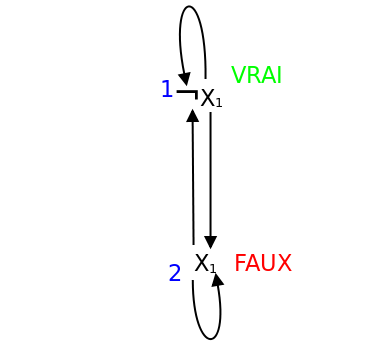
\includegraphics[height=2in, width = 3in]{img/insatisfiable.png}

%Losque l'on appiqua
%On transforme la clause $(x_{1} \vee x_{1})$ en $(\neg x_{1} \Rightarrow x_{1})$ et en 
%$(\neg x_{2} \Rightarrow x_{2})$. 

Ce graphe contient un composant fortement connexe contenant un littéral et sa négation.
La formule associée est, par conséquent, insatisfiable.

Clause contingente :  $(x_{1} \vee x_{2}) \wedge (x_{3} \vee x_{4})$	

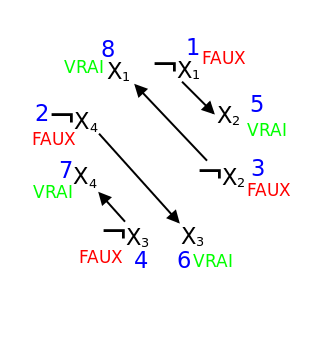
\includegraphics[height=2in, width = 3in]{img/contingente.png}

Ce graphe ne contient aucun composant fortement connexe contenant un littéral et sa négation.
Selon ces informations, la formule ci-dessus pourrait être soit contingente soit valide.

... ?? pourquoi contingente et non pas valide ??



Clause valide :  $(x_{1} \vee \neg x_{1}) \wedge (x_{2} \vee \neg x_{2})$	

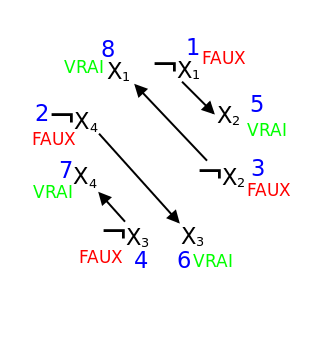
\includegraphics[height=2in, width = 3in]{img/contingente.png}



\begin{sousenonce}
Vous expliciterez ensuite l'algorithme de transformation et vous évaluerez sa complexité.
\end{sousenonce}


\begin{sousenonce}
Vous expliciterez ensuite l'algorithme d'exploration du graphe et vous évaluerez sa complexité {\it en fonction de la taille de l'ensemble de clauses initial}.
\end{sousenonce}


\begin{sousenonce}
Enfin, vous justifierez l'équivalence de la réponse au problème 2-SAT et au problème qui est posé dans le graphe.
\end{sousenonce}


\subsection{Partie Calculabilité}

\subsubsection*{Exercice \stepcounter{exocount}\bf\small \arabic{exocount} -- Sur le problème de codage}
\addcontentsline{toc}{section}{Exercice \arabic{exocount} -- Sur le problème de codage}
\setcounter{enoncecount}{0}

\begin{enonce}
Comment énumérer les couples d'entiers ?
\end{enonce}

\begin{figure}[h!]
  \centering
  \begin{tikzpicture}[
      dot/.style = {
        circle,
        fill=black,
        inner sep=0.5pt
      },
      arc/.style = {
        ->,
        >=stealth
      }
    ]
    \foreach \xpos in {0, ..., 4} {
      \foreach \ypos in {0, ..., 4} {
        \node[dot] at (\xpos,-\ypos) {};
      }
    }
    
    \draw[arc] (0,-0) -- (1,-0);
    
    \draw[arc] (1,-0) -- (0,-1);
    \draw[arc] (0,-1) -- (0,-2);
    
    \draw[arc] (0,-2) -- (1,-1);
    \draw[arc] (1,-1) -- (2,-0);
    \draw[arc] (2,-0) -- (3,-0);
    
    \draw[arc] (3,-0) -- (2,-1);
    \draw[arc] (2,-1) -- (1,-2);
    \draw[arc] (1,-2) -- (0,-3);
    \draw[arc] (0,-3) -- (0,-4);
    
    \draw[arc] (0,-4) -- (1,-3);
    \draw[arc,dashed] (1,-3) -- (2,-2);
  \end{tikzpicture}
  \caption{Graphe G}
  \label{fig:codage-zigzag}
\end{figure}

\begin{enonce}
Donner les fonctions de codage et de décodage f1(z)->x et f2(z)->y.
\end{enonce}

% TODO : John

\begin{enonce}
Montrer que l'on peut coder les triplets. Généraliser aux k-uplets, puis aux listes de longueurs quelconques.
\end{enonce}

Pour coder un triplet $(x_1, x_2, x_3)$, on code d'abord le couple $(x_1, x_2)$, puis, soit $x^*$ le résultat intermédiaire, on code le couple $(x^*, x_3)$.

\begin{figure}[h!]
  \centering
  \begin{tikzpicture}
    \node (x11) {$x_1$};
    \node[right of=x11] (x21) {$x_2$};
    \node[right of=x21] (x31) {$x_3$};
    \node[coordinate] (xmark) at ($ .5*(x11) + .5*(x21) $) {};
    \node[below of=xmark] (x*2) {$x^*$};
    \node[coordinate] (xmark2) at ($ .5*(xmark) + .5*(x*2) $) {};
    
    \node[anchor=base] (x32) at (x*2.base -| x31) {$x_3$};
    
    \node[coordinate] (xmark4) at ($ .5*(x*2) + .5*(x32) $) {};
    \node[below of=xmark4] (x*3) {résultat};
    \node[coordinate] (xmark5) at ($ .5*(xmark4) + .5*(x*3) $) {};
    
    \draw (x11) -- (xmark2);
    \draw[->] (x21) -- (xmark2) -- (x*2);
    \draw[->] (x31) -- (x32 |- x*2.north);
    \draw (x*2) -- (xmark5);
    \draw[->] (x32) -- (xmark5) -- (x*3);
  \end{tikzpicture}
  \caption{Graphe G}
  \label{fig:codage-couple}
\end{figure}

Le décodage suit tout simplement le chemin inverse (on décode ne nombre en $(x^*, x_3)$, puis on décode $x^*$ en $(x_1, x_2)$ et on recompose en $(x_1, x_2, x_3)$.

La généralisation aux k-uplets suit le même principe : On code les deux premiers nombres de la paire en nommant le résultat $x^*$, puis, on
code successivement chaque paire $(x^*, x_i)$, avec $x_i$ qui vaut successivement chaque élément du k-uplet, et $x^*$ qui vaut à chaque fois
le résultat précédent.

Le décodage d'un k-uplet de longueur k décodera le nombre en une paire $(x^*, x_i)$ $k-1$ fois, et la dernière paire ainsi générée sera
$(x_1, x_2)$. Il suffira alors de recomposer le k-uplet à partir de $x_1$, $x_2$ et tous les $x_i$.

Le codage et le décodage d'un singleton sont triviaux : $(x_1) \leftrightarrow x_1$.

Pour les listes de longueur quelconque, le problème est de savoir combien de fois faudra-t-il décoder le résultat. En effet, $(0)$, $(0,0)$
et $(0,0,0)$ ont le même code, $0$, donc il n'y a plus de bijection entre la liste et les entiers naturels, donc ambigüité lors du décodage.

Étant donné que pour un k donné, il y a une bijection entre les k-uplets et les entiers naturels, il nous suffit d'ajouter une information
permettant de déterminer de manière unique la valeur de k. On code donc d'abbord le k-uplet correspondant à la liste, en nommant le résultat
$x^*$, puis on code le couple $(x^*, k)$. Au décodage, on décodera le nombre pour obtenir $x^*$ et $k$, et on décodera $x^*$ avec la méthode
de décodage des k-uplets donnés ci-dessus.

Reste un dernier problème, celui de pouvoir encoder des listes d'entiers relatifs (et non pas juste des entiers naturels). Pour cela, on
fera une transformation préalable sur chaque élément des k-uplets :

Soit $n$ le $i$-ième élément du k-uplet, si $n$ est positif, on le transforme en le $n$-ième nombre pair, sinon, il est strictement négatif et on le transforme en le $|n|-1$ ième nombre impair. Ainsi, $0 \mapsto 0$, $1 \mapsto 2$, $2 \mapsto 4$, $-1 \mapsto 1$, $-2 \mapsto 3$, \dots

\begin{equation}
  \begin{array}{r l}
    \mathrm{transformation} : Z & \longrightarrow N \\
    n & \mapsto
    \left \{
      \begin{array}{r l}
        2n       & \text{si $n$ est pair} \\
        2(|n|-1) & \text{si $n$ est impair}
      \end{array}
    \right .
  \end{array}
\end{equation}

Le codage d'une liste d'entiers relatifs peut donc être résumé par la figure \ref{fig:codage-all}

\begin{figure}[h!]
  \centering
  \begin{tikzpicture}[
    level distance=0.7cm,
    circle,
    inner sep=0.1pt,
    ]
    \node[rectangle, inner sep=1pt] (res) {$\text{résultat}$} [grow=up]
    child[draw=red] {
      node[coordinate] (catch-k) {} edge from parent[<-]
    }
    child {
      node {x*}
      child {
        child {
          child {
            child {
              child {
                child {
                  node (xk) {$x_{\phantom{k}}$}
                  % node[anchor=base] at (xk.base) {$\vphantom{x}_{k}$}
                  % node[anchor=east] at (xk.east) {$\hphantom{x}_{k}$}
                  node[anchor=base] (get-k-v) at (xk.base) {$\vphantom{x}_{\phantom{k}}$}
                  node[anchor=east] (get-k-h) at (xk.east) {$\hphantom{x}_{\phantom{k}}$}
                  node[coordinate] (get-k-se) at (get-k-v.south -| get-k-h.east) {}
                  node[coordinate] (get-k-nw) at (get-k-v.north -| get-k-h.west) {}
                  node[anchor=base east, draw=red, inner sep=0.15pt] (the-k)
                  at (get-k-v.base -| get-k-h.east) {$\vphantom{.}_{k}$}
                }
              }
            }
          }
        } edge from parent[<-]
      }
      child {
        node {x*}
        child {
          child {
            child {
              child {
                child {node {...} edge from parent[dashed]}
                edge from parent[dashed]
              }
              edge from parent[dashed]
            }
            edge from parent[dashed]
          }
          edge from parent[dashed,<-]
        }
        child {
          node{x*}
          child {
            child {
              child {
                child {node {$x_5$}}
              }
            } edge from parent[<-]
          }
          child {
            node{x*}
            child {
              child {
                child {node {$x_4$}}
              } edge from parent[<-]
            }
            child {
              node{x*}
              child {
                child {node {$x_3$}} edge from parent[<-]
              }
              child {
                node{x*} [sibling distance=7.5mm] edge from parent[<-]
                child {node {$x_2$} edge from parent[<-]}
                child {node {$x_1$} edge from parent[<-]}
                child[missing] {}
              } edge from parent[<-]
            } edge from parent[<-]
          } edge from parent[<-]
        } edge from parent[<-]
      } edge from parent[<-]
    };
    
    \draw[red] (the-k) -| (catch-k);
    
    \node[xshift=0cm, anchor=base west] at (res.base east) {$\vphantom{\text{résultat}} = \operatorname{code}(x^*,k)$};
    
    % \node (e11) {$x_1$}; 
    % \node[right of=e11] (e21) {$x_2$};
    % \node[right of=e21] (e31) {$x_3$};
    % \node[right of=e31] (e41) {$x_4$};
    % \node[right of=e41] (e51) {$x_5$};
    % \node[right of=e51] (ed1) {\dots};
    % \node[right of=ed1] (ek1) {$x_k$};


    % \matrix[column sep=2mm, row sep=7mm]{
    %   \node (e11) {$x_1$}; & \node[coordinate] (o11) {}; &
    %   \node (e21) {$x_2$}; & \node[coordinate] (o21) {}; &
    %   \node (e31) {$x_3$}; & \node[coordinate] (o31) {}; &
    %   \node (e41) {$x_4$}; & \node[coordinate] (o41) {}; &
    %   \node (e51) {$x_5$}; & \node[coordinate] (o51) {}; &
    %   \node (ed1) {\dots}; & \node[coordinate] (o61) {}; &
    %   \node (ek1) {$x_k$}; & \node[coordinate] (o71) {}; \\
      
    %   \node[coordinate] (e12) {}; & \node (o11) {$x^*$}; &
    %   \node (e22) {$x_2$}; & \node[coordinate] (o22) {}; &
    %   \node (e32) {$x_3$}; & \node[coordinate] (o32) {}; &
    %   \node (e42) {$x_4$}; & \node[coordinate] (o42) {}; &
    %   \node (e52) {$x_5$}; & \node[coordinate] (o52) {}; &
    %   \node (ed2) {\dots}; & \node[coordinate] (o62) {}; &
    %   \node (ek2) {$x_k$}; & \node[coordinate] (o72) {}; \\
      
    %   \node[coordinate] (e12) {}; & \node[coordinate] (o12) {}; &
    %   \node[coordinate] (e22) {}; & \node (o22) {$x^*$}; & 
    %   \node (e32) {$x_3$}; & \node[coordinate] (o32) {}; &
    %   \node (e42) {$x_4$}; & \node[coordinate] (o42) {}; &
    %   \node (e52) {$x_5$}; & \node[coordinate] (o52) {}; &
    %   \node (ed2) {\dots}; & \node[coordinate] (o62) {}; &
    %   \node (ek2) {$x_k$}; & \node[coordinate] (o72) {}; \\
      
    %   \node[coordinate] (e12) {}; & \node[coordinate] (o12) {}; &
    %   \node[coordinate] (e22) {}; & \node[coordinate] (o22) {}; & 
    %   \node[coordinate] (e32) {}; & \node (o32) {$x^*$}; &
    %   \node (e42) {$x_4$}; & \node[coordinate] (o42) {}; &
    %   \node (e52) {$x_5$}; & \node[coordinate] (o52) {}; &
    %   \node (ed2) {\dots}; & \node[coordinate] (o62) {}; &
    %   \node (ek2) {$x_k$}; & \node[coordinate] (o72) {}; \\
      
    %   \node[coordinate] (e12) {}; & \node[coordinate] (o12) {}; &
    %   \node[coordinate] (e22) {}; & \node[coordinate] (o22) {}; & 
    %   \node[coordinate] (e32) {}; & \node[coordinate] (o32) {}; &
    %   \node[coordinate] (e42) {}; & \node (o42) {$x^*$}; &
    %   \node (e52) {$x_5$}; & \node[coordinate] (o52) {}; &
    %   \node (ed2) {\dots}; & \node[coordinate] (o62) {}; &
    %   \node (ek2) {$x_k$}; & \node[coordinate] (o72) {}; \\
    % };
    
    % \node[coordinate] (x11-21) at ($ .5*(x11) + .5*(x21) $) {};
    % \node[coordinate] (x21-31) at ($ .5*(x11) + .5*(x21) $) {};
    % \node[coordinate] (x31-41) at ($ .5*(x11) + .5*(x21) $) {};
    % \node[coordinate] (x41-51) at ($ .5*(x11) + .5*(x21) $) {};
    % \node[coordinate] (x51-d1) at ($ .5*(x11) + .5*(x21) $) {};
    % \node[coordinate] (xd1-k1) at ($ .5*(x11) + .5*(x21) $) {};
    
    % \node[below of=xmark] (x*2) {$x^*$};
    % \node[coordinate] (xmark2) at ($ .5*(xmark) + .5*(x*2) $) {};
    
    % \node[anchor=base] (x32) at (x*2.base -| x31) {$x_3$};
    
    % \node[coordinate] (xmark4) at ($ .5*(x*2) + .5*(x32) $) {};
    % \node[below of=xmark4] (x*3) {résultat};
    % \node[coordinate] (xmark5) at ($ .5*(xmark4) + .5*(x*3) $) {};
    
    % \draw (x11) -- (xmark2);
    % \draw[->] (x21) -- (xmark2) -- (x*2);
    % \draw[->] (x31) -- (x32 |- x*2.north);
    % \draw (x*2) -- (xmark5);
    % \draw[->] (x32) -- (xmark5) -- (x*3);
  \end{tikzpicture}
  \caption{Graphe G}
  \label{fig:codage-all}
\end{figure}

\begin{enonce}
  Peut-on énumérer les fonctions C syntaxiquements correctes ? Et les fonctions C qui ne bouclent jamais ? Justifier vos réponses le plus
  clairement et le plus synthétiquement possible.
\end{enonce}


\section{Partie pratique sur les algorithmes de flots}

\subsubsection*{Exercice \stepcounter{exocount}\bf\small \arabic{exocount} -- La méthode de Edmonds-Karp et celle de Dinic}
\addcontentsline{toc}{section}{Exercice \arabic{exocount} -- La méthode de Edmonds-Karp et celle de Dinic}
\setcounter{enoncecount}{0}

\begin{enonce}
Programmer une procédure qui construit à partir d'un graphe orienté valué (les valuations représentent les capacités) et deux sommets $s$ et $p$ du graphe, le graphe d'écart associé (correspondant à un flot nul sur chaque arc).
\end{enonce}


\begin{enonce}
Programmer un procédure qui à partir d'un graphe orienté et deux sommets $s$ et $p$ donne un plus court chemin en nombre d'arcs de $s$ à $p$ ou qui signale s'il n'y en a pas.
\end{enonce}


\begin{enonce}
Etant donnés un graphe G orienté et valué et un chemin de G, écrire une fonction uqi calcule l'arc de plus petite valuation sur le chemin.
\end{enonce}


\begin{enonce}
Etant donnés un graphe d'écard, un chemin et un entier $k$, donner une procédure qui met à jour le graphe d'écard si on augmente le flot de $k$ le long de la chaîne augmentante correspondant au chemin. 
\end{enonce}


\begin{enonce}
Ecrire une procédure qui à partir du graphe initial et du graphe d'écard final (plus de chemins entre $s$ et $p$ donne la valeur du flot maximum ainsi que la valeur deu flot sur chaque arc lorsque le flot maximum est atteint. 
\end{enonce}


\begin{enonce}
En utilisant les procédures et les fonctions précédentes, programmer l'algorithme de Edmond-Karp. 
\end{enonce}


\begin{enonce}
Ecrire une procédure qui prend en compte l'ensemble des plus cours chemins en nombres d'arcs.
\end{enonce}


\begin{enonce}
Ecrire une procédure qui calcule la plus petite valeur du flot dans le graphe de couche.
\end{enonce}


\begin{enonce}
Ecrire une procédure qui met à jour le flot dans le graphe G. 
\end{enonce}


\begin{enonce}
En déduire l'algorithme de Dinic.
\end{enonce}


\begin{enonce}
Comparer les résultats (temps d'exécution, taux d'occupation mémoire) entre les deux méthodes. Vous apporterez un soin tout particulier à la génération de vos résultats et à leur présentation.
\end{enonce}

\end{document}
